%%%%%%%%%%%%%%%%%%%%%%%%%%%%%%%%%%%%%%%%%
% Original author of template for CV (Plasmati Graduate CV v1.0 24/03/2013):
%  Alessandro Plasmati (alessandro.plasmati@gmail.com)
% Downloaded from:
%  http://www.LaTeXTemplates.com
% Modifications by:
%  Pol del Aguila Pla (polsocjo@gmail.com)
% License:
%  CC BY-NC-SA 3.0 (http://creativecommons.org/licenses/by-nc-sa/3.0/)
% Important note:
%  This template needs to be compiled with XeLaTeX.
%  The main document font is called Fontin and can be installed in sudo-enabled
%  Linux systems by running fixFONTproblem.sh (will internally call sudo when necessary).
%%%%%%%%%%%%%%%%%%%%%%%%%%%%%%%%%%%%%%%%%

%----------------------------------------------------------------------------------------
%	PACKAGES AND OTHER DOCUMENT CONFIGURATIONS
%----------------------------------------------------------------------------------------

% Font and paper size
\documentclass[a4paper,10pt]{article}

% Font loading
\usepackage{fontspec} 
  \defaultfontfeatures{Mapping=tex-text}
  % Set main font for document
  \setmainfont[SmallCapsFont = Fontin SmallCaps]{Fontin} 

% Formatting
\usepackage{xunicode,xltxtra,url,parskip} 

% Coloring
\usepackage[usenames,dvipsnames]{xcolor} 

% Margin specification
\usepackage{fullpage}

% Links and other clickable references
\usepackage{hyperref} 
  % Link colors
  \definecolor{linkcolour}{rgb}{0,0.2,0.6}
  \hypersetup{colorlinks,breaklinks,urlcolor=linkcolour,linkcolor=linkcolour}

% Costumize section command
\usepackage{titlesec} % Used to customize the \section command
  % Text formatting
  \titleformat{\section}{\Large\scshape\raggedright}{}{0em}{}[\titlerule]
  % Spacing
  \titlespacing{\section}{0pt}{3pt}{3pt}

% Insert images
\usepackage{graphicx}

% Footnotes in tables
\usepackage{footnote}

\begin{document}

  % Remove page numbers
  \pagestyle{empty}

  %----------------------------------------------------------------------------------------
  %	NAME AND CONTACT INFORMATION
  %----------------------------------------------------------------------------------------

  \begin{center}
    \begin{tabular}{lcr}
	    \par{\centering{\Huge Pol \textsc{del Aguila Pla}}\bigskip\par} & & 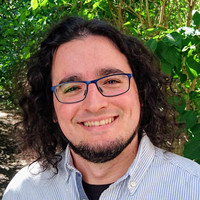
\includegraphics[width=0.3\textwidth]{../main/pol.jpg} \\
    \end{tabular}
  \end{center}
  
  \section{Personal data}
  
    \begin{tabular}{rl}
      \textsc{Place and date of birth:} & Barcelona, Catalonia, on 13 September 1990 \\
      \textsc{Home address:} & Carl Malmstens v\"{a}g 8, Lgh 1103, Solna, Sweden \\
      \textsc{Mobile phone:} & +46 (0)7-294-2302 \\
      \textsc{Email:} & \href{mailto:poldap@kth.se}{\nolinkurl{poldap@kth.se}} \\
      \textsc{Website:} & \href{https://poldap.github.io}{\url{poldap.github.io}}
    \end{tabular}

%----------------------------------------------------------------------------------------
%	WORK EXPERIENCE 
%----------------------------------------------------------------------------------------

  \section{Research Experience}
  
    \begin{tabular}{r|p{13cm}}
    
      \textsc{2019 Aug} 	& Ph.D. Thesis [Expected] \\
      \textsc{2014 Sept} 	& \emph{Signal processing and non-linear modeling} \\
				& \footnotesize{ \textbf{Department of Information Science and Engineering}, School of Electrical Engineering and Computer Science,
				  KTH Royal Institute of Technology, Stockholm, Sweden.} \\
      \multicolumn{2}{c}{} \\

      \textsc{2014 Sept} 	& Research Engineer \\
      \textsc{2014 Mar} 	& \emph{Probability density estimation, a review of the state of the art.} \\ 
				& \footnotesize{ \textbf{Department of Signal Processing}, School of Electrical Engineering,
				  KTH Royal Institute of Technology, Stockholm, Sweden.} \\
      \multicolumn{2}{c}{} \\
      %------------------------------------------------

      \textsc{2014 Mar} 	& Master's thesis \\
      \textsc{2013 Aug} 	& \emph{ Normalization of remote sensing imagery for automatic information extraction } \\ 
				& \footnotesize{ \textbf{Department of Communication Theory}, School of Electrical Engineering,
				  KTH Royal Institute of Technology, Stockholm, Sweden.} \\
      \multicolumn{2}{c}{} \\

      %------------------------------------------------

      \textsc{2012 Aug} 	& Undergraduate research \\
      \textsc{2012 Apr} 	& \emph{Image analysis for sport events classification, a review of the state of the art.} \\ 
				& \footnotesize{ \textbf{Image Processing Group (GPI)}, Department of Signal Theory and 
				  Communications (TSC), \emph{Escola T\`{e}cnica Superior d'Enginyeria de Telecomunicaci\'{o} 
				  de Barcelona}, UPC BarcelonaTech.} \\

    \end{tabular}

  %----------------------------------------------------------------------------------------
  %	EDUCATION
  %----------------------------------------------------------------------------------------

  \section{University education}

    \begin{tabular}{r|p{13cm}}	
    
      \textsc{2014 Mar}  & \emph{Civilingenj\"{o}r}, 5-year degree in \textbf{Electrical Engineering} \\
      \textsc{2012 Aug}  & \footnotesize{\textbf{KTH Royal Institute of Technology}, Stockholm, Sweden. 
			   Heavily specialized in signal processing and its applications to communications and imaging. Double degree program.} \\ 
      \multicolumn{2}{c}{} \\

      %------------------------------------------------
      
      \textsc{2014 Mar}  & \emph{Enginyer de Telecomunicaci\'{o}}, 5-year degree in \textbf{Telecommunications Engineering} \\  
      \textsc{2008 Sep}  & \footnotesize{\textbf{UPC BarcelonaTech}, \emph{Universitat Polit\`{e}cnica de Catalunya, Escola T\`{e}cnica Superior
			   d'Enginyeria de Telecomunicaci\'{o} de Barcelona}, Barcelona, Catalonia. 
			   Specialized in signal processing and its applications to pattern recognition and speech processing. Double degree program.} \\
    \end{tabular}

  %----------------------------------------------------------------------------------------
  %	PUBLICATIONS
  %----------------------------------------------------------------------------------------
    \renewcommand\refname{Publications}
    \nocite{AguilaPla2017,AguilaPla2017a,AguilaPla2018,AguilaPla2018a,AguilaPla2014,Mabtech2017}
    \bibliographystyle{IEEEtran_Pol}
    \bibliography{../pubs/bibfile}
	
  %----------------------------------------------------------------------------------------
  %	SCHOLARSHIPS AND ADDITIONAL INFO
  %----------------------------------------------------------------------------------------

  \section{Grants and awards}
    \begin{savenotes}
    \begin{tabular}{r|p{13cm}}
      
      \textsc{2018 Jun} & Travel grants. Total amount of $43000\,\mathrm{SEK}$.\\
      \textsc{2017 Sep} & \footnotesize{\textbf{KTH Opportunities Fund} project scholarship,
			  \textbf{Knut and Alice Wallenberg Jubilee appropriation} travel grant,
			  \textbf{\AA forsk Foundation} travel grant and 
			  \textbf{Engineering Sciences 2017 call from The Royal Swedish
			  Academy of Sciences (KVA, call ES2017-0011)} project and travel 
			  grant.} \\
      \multicolumn{2}{c}{} \\
      
      \textsc{2013 Mar} & Exchange studies scholarships \\ 
      \textsc{2012 Aug} & \footnotesize{\textbf{Erasmus} and \textbf{AGAUR}\footnote{Catalan University and Research Scholarships Agency} exchange studies scholarships.}  \\
      \multicolumn{2}{c}{} \\

      \textsc{2009 Jun}	& Promotion's top-10 award. Ranked $4^{\mathrm{th}}$. \\
      \textsc{2008 Sep}	& \footnotesize{Receiver of the UPC BarcelonaTech award for \textbf{first 
			  year students with top-10 grades} in Telecommunications Engineering.} \\

    \end{tabular}
    \end{savenotes}

  %----------------------------------------------------------------------------------------
  %	Contact with the scientific community
  %----------------------------------------------------------------------------------------
  
  \section{International participation in the scientific community}

    \begin{tabular}{r|p{13cm}}
      
      \textsc{2018 Jun} & Poster presentation within the \emph{SIAM Conference on Imaging Science}
			  (SIAM-IS 2018), titled \textbf{Source localization by spatially
			  variant blind deconvolution}. \\
			& \footnotesize{University of Bologna, Bologna, Italy.}\\
      \multicolumn{2}{c}{} \\
    
      \textsc{2018 Apr} & Poster presentation within the \emph{IEEE International Conference 
			  on Acoustics, Speech and Signal Processing} (ICASSP 2018), titled
			  \textbf{Convolutional group-sparse coding and source localization}. \\
			& \footnotesize{Calgary Talus Convention Centre, Calgary, Alberta, Canada.} \\
			& \\
			& Poster presentation within the \emph{2018 IEEE $15^{\mathrm{th}}$ International
			  Symposium on Biomedical Imaging} (ISBI 2018), titled
			  \textbf{Cell detection on image-based immunoassays}.\\
			& \footnotesize{Omni Shoreham Hotel, Washington, D.C., United States of America.} \\
      \multicolumn{2}{c}{} \\
      
      \textsc{2017 Nov} & Oral presentation within the workshop \emph{Generative models, 
			  parameter learning, and sparsity} (VMVW02), titled
			  \textbf{Cell detection by functional inverse diffusion and group sparsity},
			  access at \url{https://downloads.sms.cam.ac.uk/2600830/2600858.mp4}. \\
			& \footnotesize{\textbf{Isaac Newton Institute for Mathematical Sciences},
			  \textbf{University of Cambridge}, Cambridge, United Kingdom.
			  Within the programme \emph{Variational methods and effective
			  algorithms for imaging and vision}.}\\
      \multicolumn{2}{c}{} \\
      
      \emph{Current}	& Reviewer for the IEEE Transactions on Signal Processing \\
      \textsc{2015 Aug} & \footnotesize{Reviewed \textbf{2 articles} for the journal.} \\
      
    \end{tabular}

%----------------------------------------------------------------------------------------
%	REFERENCES
%----------------------------------------------------------------------------------------
% \section[title]{References }
% \begin{center}
% \begin{tabular}{lccc}
% Name & \textsc{\href{https://imatge.upc.edu/web/ferran}{Dr. Ferran Marqués}} & \textsc{\href{https://spcom.upc.edu/index.php?option=com_spcom\&Itemid=3\&id=24}{Dr. Josep Vidal}}  & \textsc{\href{http://www.csc.kth.se/~johnf/}{Dr. John Folkesson}}\\
% Group & \textsc{\href{http://imatge.upc.edu}{GPI}} & \textsc{\href{http://spcom.upc.edu}{SPCOM}} & \textsc{\href{http://www.kth.se/en/csc/forskning/cas}{CAS}} \\ 
% Department & \textsc{\href{http://www.tsc.upc.edu/en}{TSC}} & \textsc{\href{http://www.tsc.upc.edu/en}{TSC}} & \textsc{CSC}\\  
% University & \textsc{UPC} & \textsc{UPC}  & \textsc{KTH}\\
% Email & \href{mailto:ferran.marques@upc.edu}{ferran.marques@upc.edu} & \href{mailto:josep.vidal@upc.edu}{josep.vidal@upc.edu} & \href{mailto:johnf@csc.kth.se}{johnf@csc.kth.se} \\
% Telephone & +34 93 401 68 32 & + 34 93 401 64 57  & +46 (0)8-790-6201 \\
% \multicolumn{4}{c}{}\\
% \end{tabular}

% 
% \begin{tabular}{lcc}
% Name & \textsc{Dr. Juan-Manuel Rius Casals}& \textsc{Dr. Antonio Bonafonte}  \\
% Group & \textsc{\href{http://www.tsc.upc.edu/antennalab/}{AntennaLab}} & \textsc{\href{http://www.talp.upc.edu}{TALP}} \\
% Department & \textsc{\href{http://www.tsc.upc.edu/en}{TSC}}  & \textsc{\href{http://www.tsc.upc.edu/en}{TSC}}\\
% University & \textsc{UPC} & \textsc{UPC} \\
% Email & \href{mailto:rius@tsc.upc.edu}{rius@tsc.upc.edu}  & \href{mailto:antonio.bonafonte@upc.edu}{antonio.bonafonte@upc.edu}\\
% Telephone & +34 93 401 72 19 & + 34 93 401 07 64 \\
% 
%  
% \end{tabular}
% 
% \end{center}


  %----------------------------------------------------------------------------------------
  %	LANGUAGES
  %----------------------------------------------------------------------------------------

  \section{Languages}

    \begin{tabular}{rl}
      
      \textsc{Mother tongue:} & Catalan and Spanish \\
      
      \textsc{Professional:} & English \\
      
      \textsc{Conversational:} & Swedish \\
      
      \textsc{Basic:} & Italian and French (\textsc{DELF} A-2, \textsc{2006 Aug})
      
    \end{tabular}

  %----------------------------------------------------------------------------------------
  %	COMPUTER SKILLS 
  %----------------------------------------------------------------------------------------

  \section{Technical and Computer Skills}

  \begin{tabular}{rl}
  Technical skills: & Electronic design and measurement, network testing and \\
  & simulation, use of vector signal analysers for digital  \\
  & communications, Antenna design and performance analysis. \\
  &\\
  Computer skills:& Comfortable performing administrative tasks \\
  & in both Linux and Windows environments. \\
  &\\
  Programming languages: & \textsc{C, Java, Matlab, Bash } \\

  \end{tabular}


%----------------------------------------------------------------------------------------
%	INTERESTS AND ACTIVITIES
%----------------------------------------------------------------------------------------

\section{Interests and Activities}

Linux and Open Source community \\
Writing short stories\\
Hiking, skiing, cycling, skating and capoeira

%----------------------------------------------------------------------------------------


\end{document}
